\documentclass{beamer}
\usetheme{boxes}
\usepackage[ scaled ]{ helvet }
%This removes an error message.
\let\Tiny=\tiny

\newcommand{\bF}{{\mathbb{F}}}
\newcommand{\bQ}{{\mathbb{Q}}}
\newcommand{\bZ}{{\mathbb{Z}}}

\renewcommand{\P}{{\mathcal{P}}}

\newcommand{\tor}{\textnormal{tor}}

\renewcommand{\mod}[1]{{\ifmmode\text{\rm\ (mod~$#1$)}\else\discretionary{}{}{\hbox{ }}\rm(mod~$#1$)\fi}}
\newcommand{\legendre}[2]{\genfrac{(}{)}{}{}{#1}{#2}}

\setbeamertemplate{navigation symbols}{}

\title[The Math Educational Resources Wiki]{{\bf\Huge The Math Educational \\[.25cm] Resources Wiki}}
\institute{The University of British Columbia}
\author{{\small Carmen Bruni, Christina Koch, Bernhard Konrad, Michael Lindstrom, Iain Moyles and William Thompson\\
On behalf of the entire MER wiki team}}
\date{
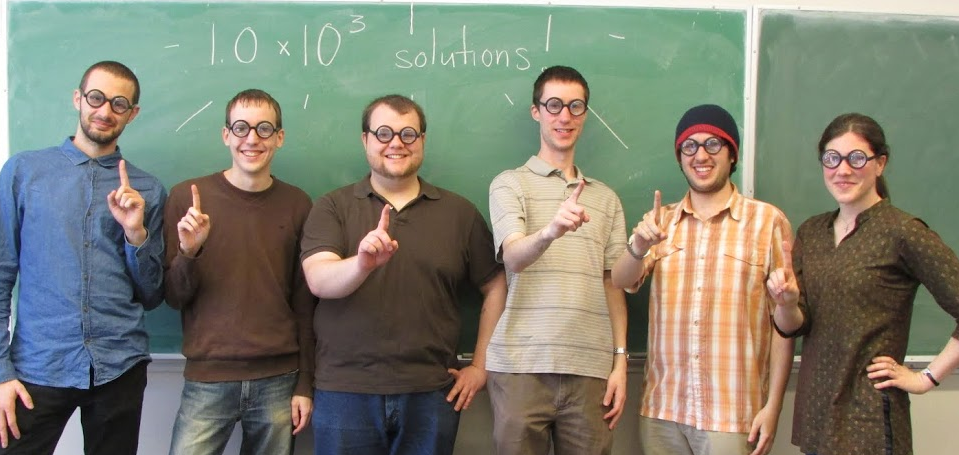
\includegraphics[width=0.7\textwidth]{MER_nerds.png}
}
%
\includegraphics[width=0.34\textwidth]{David_Webster.jpg}\hspace{1em}

\hypersetup{colorlinks=true, linkcolor=cyan, urlcolor=cyan}
\begin{document}

\frame{ \titlepage }

\frame{
\frametitle{\bf{Our Resource}}
\begin{center}
{\tt http://wiki.ubc.ca/Science:Math\_Educational\_Resources}
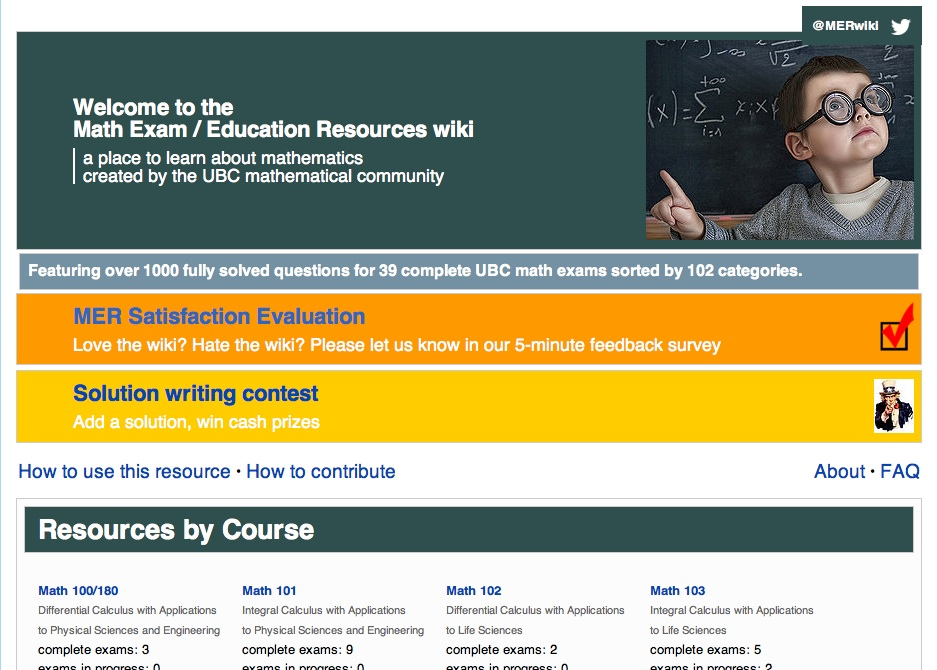
\includegraphics[width=\textwidth]{frontpage3.jpg}
\end{center}
}

\frame
{
\frametitle{\bf{Brief History of the MER Wiki}}

  \begin{block}{}

      \begin{itemize}
      \item Math Department makes past exams publically available.
      \item Previous to the wiki, exam solution packages were printed off in hard copy and sold to students.
      \item In February 2012 math graduate students decided to collaborate and make the solutions to these exams free to students.
      \item Our goal: improve quality of content, system of content delivery, allow student interaction.
	  \item The wiki structure is easy for new contributors, great to work collaboratively and intuitive to use.

      \end{itemize}
\end{block}
}



\frame{
\frametitle{\bf{Achievements and Vision}}
    \begin{block}{How far has this volunteer effort come in two years?}
        \begin{itemize}
            \item 40 complete exams, over 1000 fully written hints and solutions from about 35 contributors.
            \item Added several dynamic and interactive features over time, like tagging system, course syllabus, rating bar, videos, and more.
            \item Extensive student usage - over 800,000 views!
        \end{itemize}
    \end{block}
    %\includegraphics[scale=0.3]{total_clicks_in_term.jpg}

\begin{block}{Our Vision}
\begin{itemize}
\item Make this the best learning resource possible for undergraduate students taking math courses at UBC.

\item Support instructors in the UBC Math Department.

\item Be a role model for similar initiatives in other departments.
\end{itemize}
\end{block}
}



\frame{
\frametitle{\bf More Than 1000 Exam Pages Like This One!}
\noindent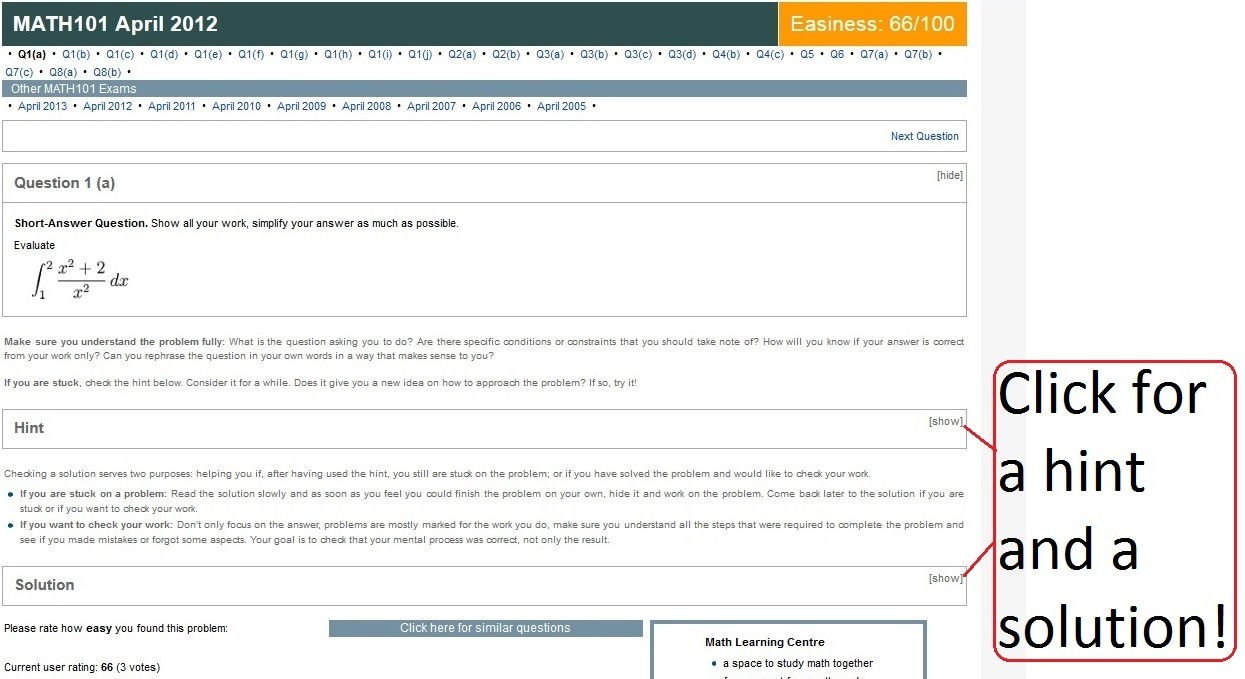
\includegraphics[width=\textwidth]{QuestionPage5.jpg}
}

\frame
{\frametitle{\bf{Peer Reviewed Content}}

All content is peer reviewed. This is a \emph{common workflow:}

\medskip

\begin{itemize}
\item \textbf{Contributor A}: Adds question statement.
\item \textbf{Contributor B}: Reviews question statement. Also adds hint and solution.
\item \textbf{Contributor A}: Approves the hint, leaves a note on the discussion page that the solution should be more clear.
\item \textbf{Contributor C}: Edits solution.
\item \textbf{Contributor A}: Approves edited solution.
\end{itemize}
}



\frame
{\frametitle{{\bf Student Interaction}}

\begin{columns}
\begin{column}{0.3\textwidth}
Students suggest corrections and alternate solutions:
\newline
\vspace{4em}

Students can also ask for clarification to improve their understanding:
\end{column}
\begin{column}{0.7\textwidth}
%\includegraphics[scale=0.3]{suggestion.png}
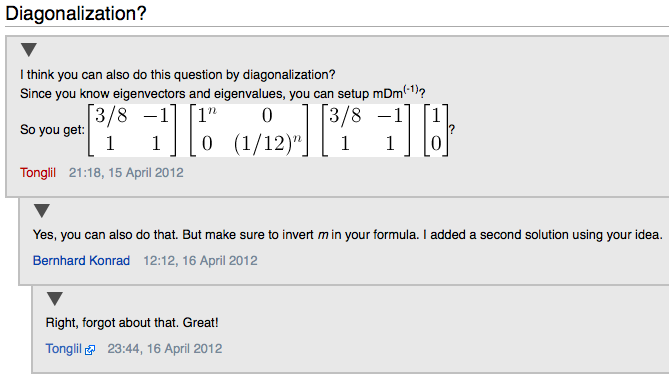
\includegraphics[width=\textwidth]{diagonalization.png}
\hrule
\smallskip
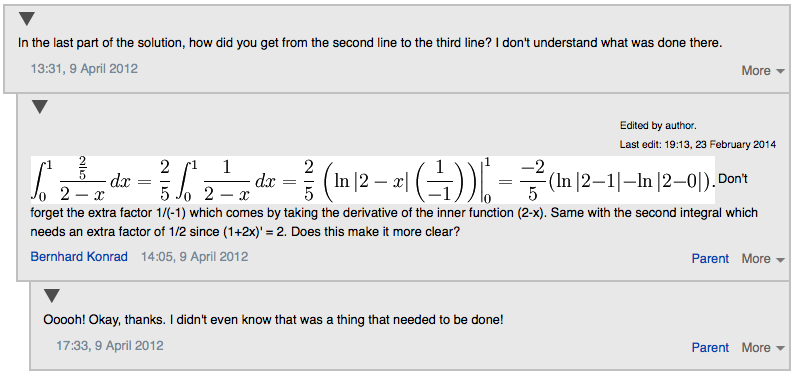
\includegraphics[width=\textwidth]{CommentQuestion3.png}
\end{column}
\end{columns}

}

\frame
{\frametitle{\bf{Tagging by Topic}}
\begin{columns}
\begin{column}{0.6\textwidth}
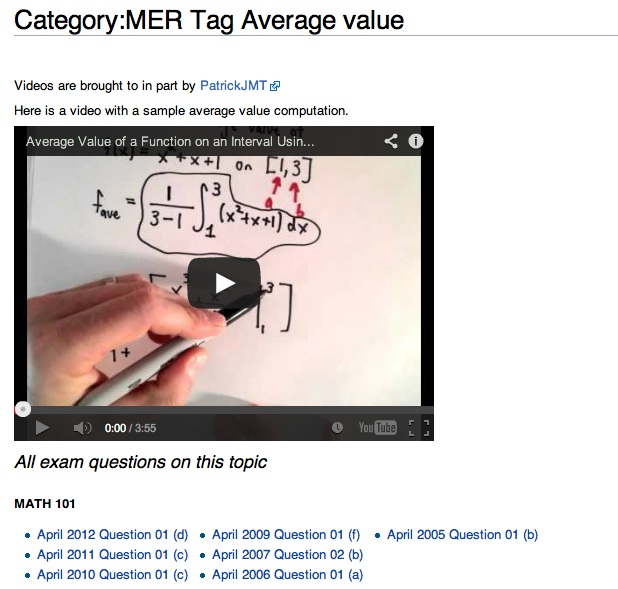
\includegraphics[width=\textwidth]{tag_with_video2.jpg}
\end{column}
\begin{column}{0.4\textwidth}
Individual exam questions are tagged by topic.

\medskip

Most topic pages contain instructional videos (from PatrickJMT on YouTube).

\medskip

All relevant exam questions across all courses are listed.
\end{column}
\end{columns}
}

\frame
{\frametitle{\bf{Dynamic Syllabus}}
%\begin{columns}
%\begin{column}{0.65\textwidth}
\begin{center}
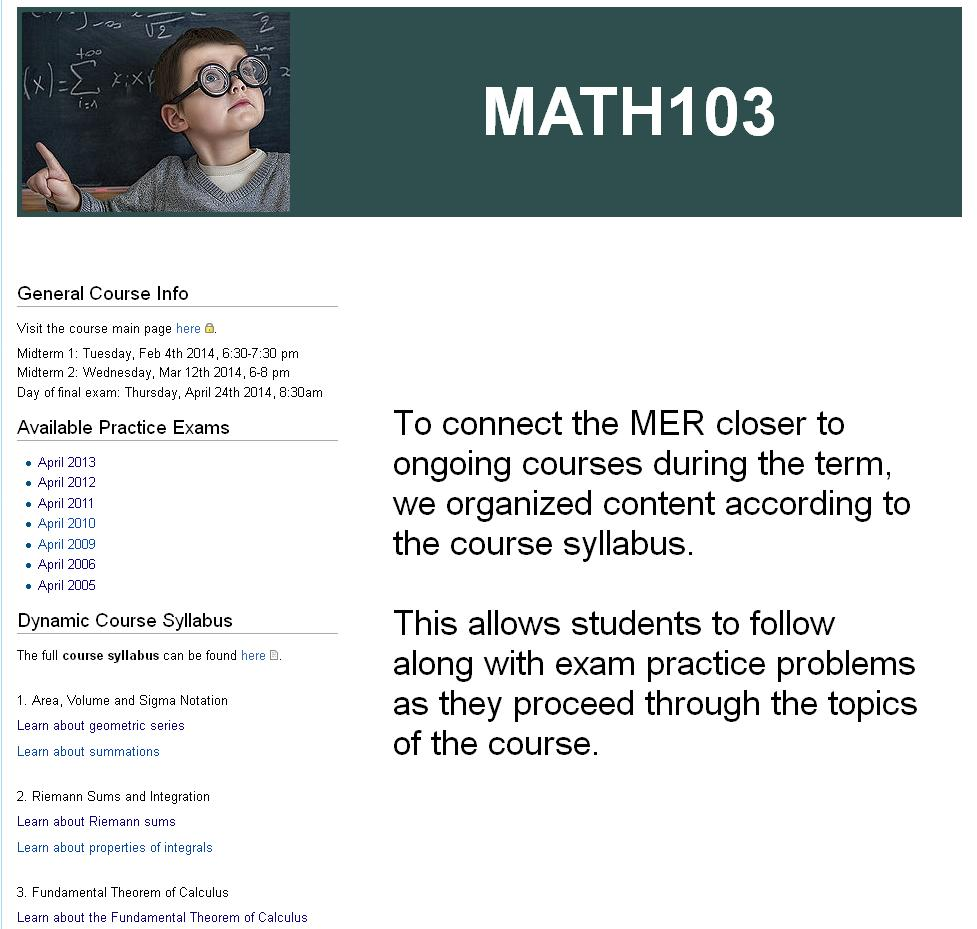
\includegraphics[scale = 0.3]{DynamicSyllabus.JPG}
\end{center}
%\end{column}
%\begin{column}{0.35\textwidth}
%To connect the MER closer to ongoing courses during the term, we organized content according to the course syllabus.

%\medskip

%This allows students to follow along with exam practice problems as they proceed through the topics of the course.
%\end{column}
%\end{columns}
}

\frame
{\frametitle{\bf{Student Tag Use}}
\begin{columns}
\begin{column}{0.6\textwidth}
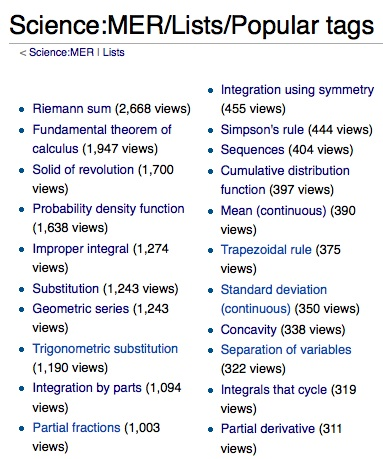
\includegraphics[width=\textwidth]{popular_tags2.jpg}
\end{column}
\begin{column}{0.4\textwidth}
For the Jan. - Apr. 2014 term we implemented the dynamic syllabus and fully tagged questions. Student use is reflected in the number of views per tag.

\medskip

The most popular tags all pertain to integral calculus, suggesting that students studied for their classes and midterms using the appropriate topic tags.
\end{column}
\end{columns}
}


\frame
{\frametitle{\bf{The Rating Bar}}
\begin{columns}
\begin{column}{0.4\textwidth}
At the bottom of every question a rating bar asks students to vote on how easy they perceive the problem.
\medskip
\hrule
\smallskip
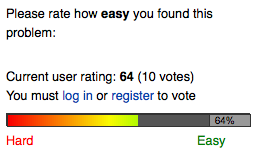
\includegraphics[width=\textwidth]{ratingBar.png}
\end{column}
\begin{column}{0.6\textwidth}
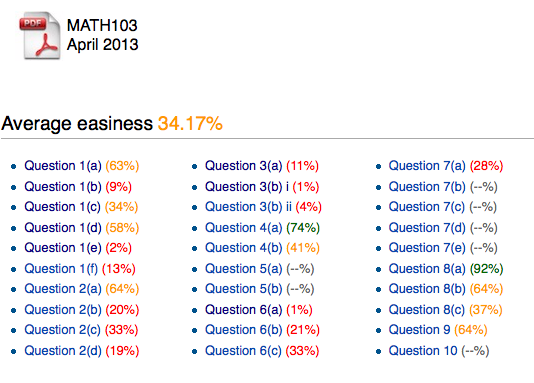
\includegraphics[width=\textwidth]{M103_exampage.png}
\end{column}
\end{columns}
\smallskip
This rating can then be used by other students to help sort exam questions by easiness and it can help instructors by suggesting problems/topics for future exams that give balanced difficulty.
}



\frame
{\frametitle{\bf{Our Latest Features}}
\begin{columns}
\begin{column}{0.33\textwidth}
{\bf \color{blue} Additional help}\\[.25cm]
Each question page informs about additional help in the Math Departments Leaning Centre or finding a private tutor.
\medskip
\hrule
\bigskip


\includegraphics[width=\textwidth]{additional_help.png}
\end{column}
\begin{column}{0.33\textwidth}
\raisebox{-.55cm}{
{\bf \color{blue} Android App}
}

\vspace{-.1cm}
\begin{center}

\includegraphics[width=.6\textwidth]{en_app_rgb_wo_45.png}

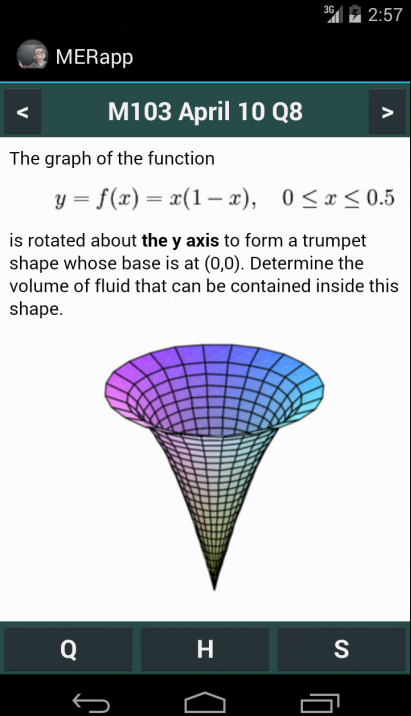
\includegraphics[width=\textwidth]{app_screen.png}
\end{center}
\end{column}
\begin{column}{0.33\textwidth}
\raisebox{2.65cm}{
{\bf \color{blue} Solution contest}
}

\vspace{-1.8cm}
In a solution writing contest students can suggest solutions and win cash prizes.

\bigskip
\hrule
\bigskip
{\bf \color{blue} Exam prep sessions}\\[.25cm]
For the April 2014 exam period we offer free prep sessions on general study tips and how to use the wiki most effectively.
\end{column}
\end{columns}
}



\frame
{\frametitle{\bf{General Usage Data}}

This graph displays total clicks per day over the lifespan of the MER wiki.

\smallskip

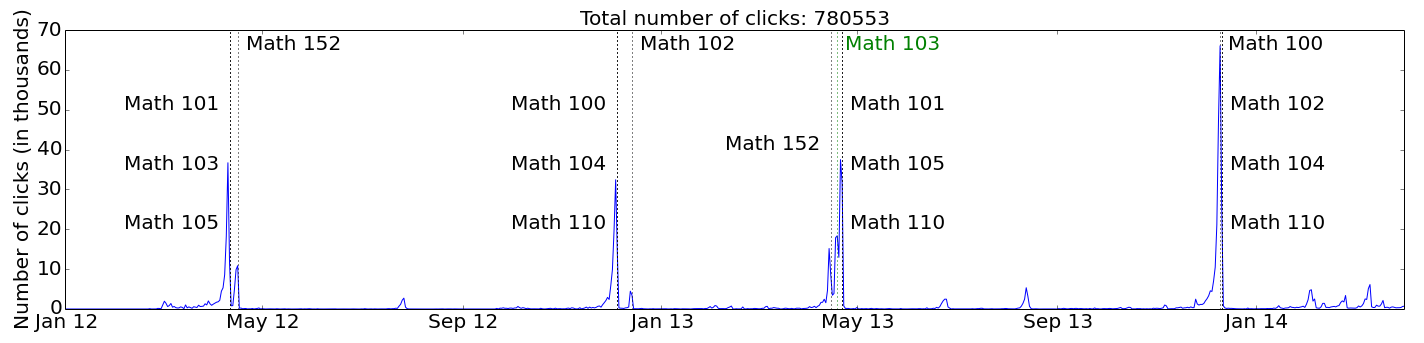
\includegraphics[width=\textwidth]{spikes2.png}

\smallskip

Usage spikes in a big way around exam time! Can you guess when summer school exams were held?

\medskip

Notice that there are new bumps near midterm time in February and March 2014. This is because students use the dynamic syllabus to study by topic, not just around final exam time.

}

\frame
{\frametitle{{\bf More Detailed Google Analytics Data}}
\begin{columns}
    \begin{column}{0.45\textwidth}
        We also determined the breakdown of time spent per course, and per exam by course (among other things).  \newline \\ This information can help tell us about student study habits.
    \end{column}
    \begin{column}{0.55\textwidth}
        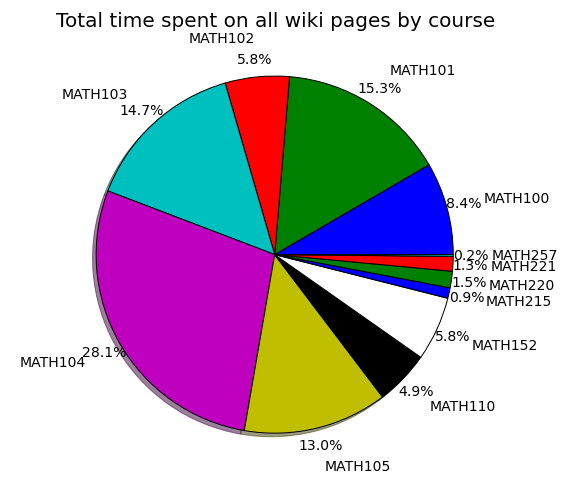
\includegraphics[width=\textwidth]{course_time2.png}
    \end{column}
\end{columns}
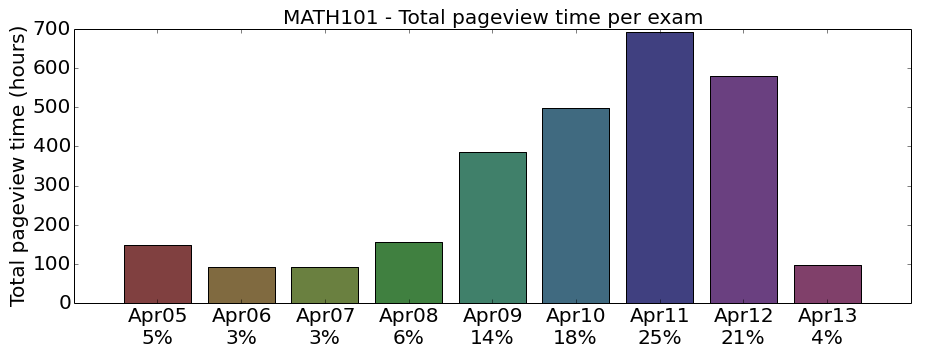
\includegraphics[width=0.8\textwidth]{exams_101only2.png}
}

%%%Condense the following three slides into one
\frame
{
  \frametitle{\bf{Research on worked examples}}

\alert{Question:} Are worked examples useful for students or harmful?

\medskip

Research suggests that
            \begin{enumerate}
            \item Students who see worked examples and conventional problems versus only seeing conventional problems do better on test questions containing similar problems (Sweller-Cooper '85), (Cooper-Sweller '87), (Paas-Van Merri\"enboer '94).
            \item Students also spend less time on worked examples than on conventional problems (S-C '85), (C-S '87), (P-V M '94).
            \item Students who are in the worked example group also can perform better and spend less time on transfer problems (that is, examples not identical to the practice ones) provided the variance in difficulty is not too large (C-S-V  '87), (P-V M'94)
            \end{enumerate}
}

%\frame
%{
%  \frametitle{Research on worked-examples}

            %\begin{enumerate}
            %\setcounter{enumi}{2}
            %\item Students who are in the worked example group also can perform better and spend less time on transfer problems (that is, examples not identical to the practice ones) provided the variance in difficulty is not too large (C-S '87), (P-V M '94).
            %\item Strong students are not effected by the type of practice so long as they spend ``enough time'' on task. Weak students however perform much better on tests provided they have spent enough time on worked examples  (C-S '87).
            %\end{enumerate}
%}

%\frame
%{
%  \frametitle{Research on worked-examples}

%            \begin{enumerate}
%            \setcounter{enumi}{4}
%            \item When normalized for time, students perform substantially better and are faster on transfer problems than a conventional problem group (C-S '87).
%            \item Students seeing worked examples on problems of large variability will in general perform better on transfer tests (P-V M '94). \pause
%            \end{enumerate}

%          \alert{Summary: Students need to develop schemata for organizing problems which can be faciliated by worked examples.}
%}

\frame
{ \frametitle{\bf{Moving Forward}}
    \begin{block}{Possible future directions}
      \begin{itemize}
            \item Add non-exam questions and ``fill in the details'' solutions.
            \item Complete and develop the topic tagging structure.
            \item Increase sustainability.
       \end{itemize}
    \end{block}
    \begin{block}{Funding through TLEF}
        \begin{itemize}
            \item Evaluate effectiveness of resource through surveys and interviews.
            \item Add features as suggested by the above evaluation.
       \end{itemize}
    \end{block}

\emph{We are very thankfull to Warren Code, Eric Cytrynbaum, Will Engle, Gillian Gerhard, Wes Maciejewski, Scott McMillan, Cindy Underhill, and the CTLT IT team for ongoing support and advice.}
}
\end{document}

%sagemathcloud={"zoom_width":105}